\section{Feature use in sampled forests}
\label{app:candidate-availability}

\Cref{fig:candidate-dimension-curves,fig:regression-candidate-dimension-curves}
extend the feature-use measurement of \cref{sec:mechanism} to
$p \in \{100,500,1{,}000\}$, for classification and regression separately.
Each forest uses 1,000 trees per fit. For each method and feature dimension $p$, each point is the mean over
$n_{\mathrm{informative}} \in \{1,2,5,10\}$, and the capped bar spans the
minimum and maximum over those four sparse settings. The values quoted below
for designs with one, two, or five informative features are single-design
values from the same runs, not read from the plotted means.

In classification, evaluating all nonconstant features at each split gives the
largest informative-feature gains in sparse high-$p$ settings. CIF-all isolates
feature subsampling because feature muting and the other tree settings are held
fixed. Averaged over the 12 classification designs, CIF uses
informative features in 33.2\% of splits and CIF-all in 91.7\%, and CIF uses
more distinct uninformative features, a mean of 265.1 against 93.4, where each
count is the number of distinct uninformative features used anywhere in the
five pooled fits of a design. With two informative features and $p{=}100$, CIF uses informative
features in 40.0\% of splits, while CIF-all does so in 100.0\%.
The corresponding values are 12.2\% versus 90.2\% at $p{=}500$ and 9.0\% versus
100.0\% at $p{=}1{,}000$, and in those three designs CIF-all uses 70, 264, and
439 fewer distinct uninformative features than CIF (totals over the pooled
fits). With five informative features, the CIF-all
minus CIF differences are 25.1, 56.4, and 54.3\%
at $p{=}100$, $p{=}500$, and $p{=}1{,}000$.

Regression shows a similar informative-feature use pattern in the one-
and two-informative-feature settings, and there CIF-all uses more distinct
uninformative features than CIF. Averaged over the regression designs, CIF-all
uses informative features in 42.3\% of splits against 27.8\% for CIF, and a
mean of 528.8 distinct uninformative features against 367.7. With two informative features and $p{=}100$, CIF uses
informative features in 39.9\% of splits, while CIF-all does so in 58.8\%.
The corresponding values are 19.7\% versus 46.7\% at $p{=}500$ and 11.6\%
versus 35.9\% at $p{=}1{,}000$. With one informative feature, the CIF-all minus
CIF differences are 29.8, 18.9, and 42.1\%.

\begin{figure}[!htbp]
  \centering
  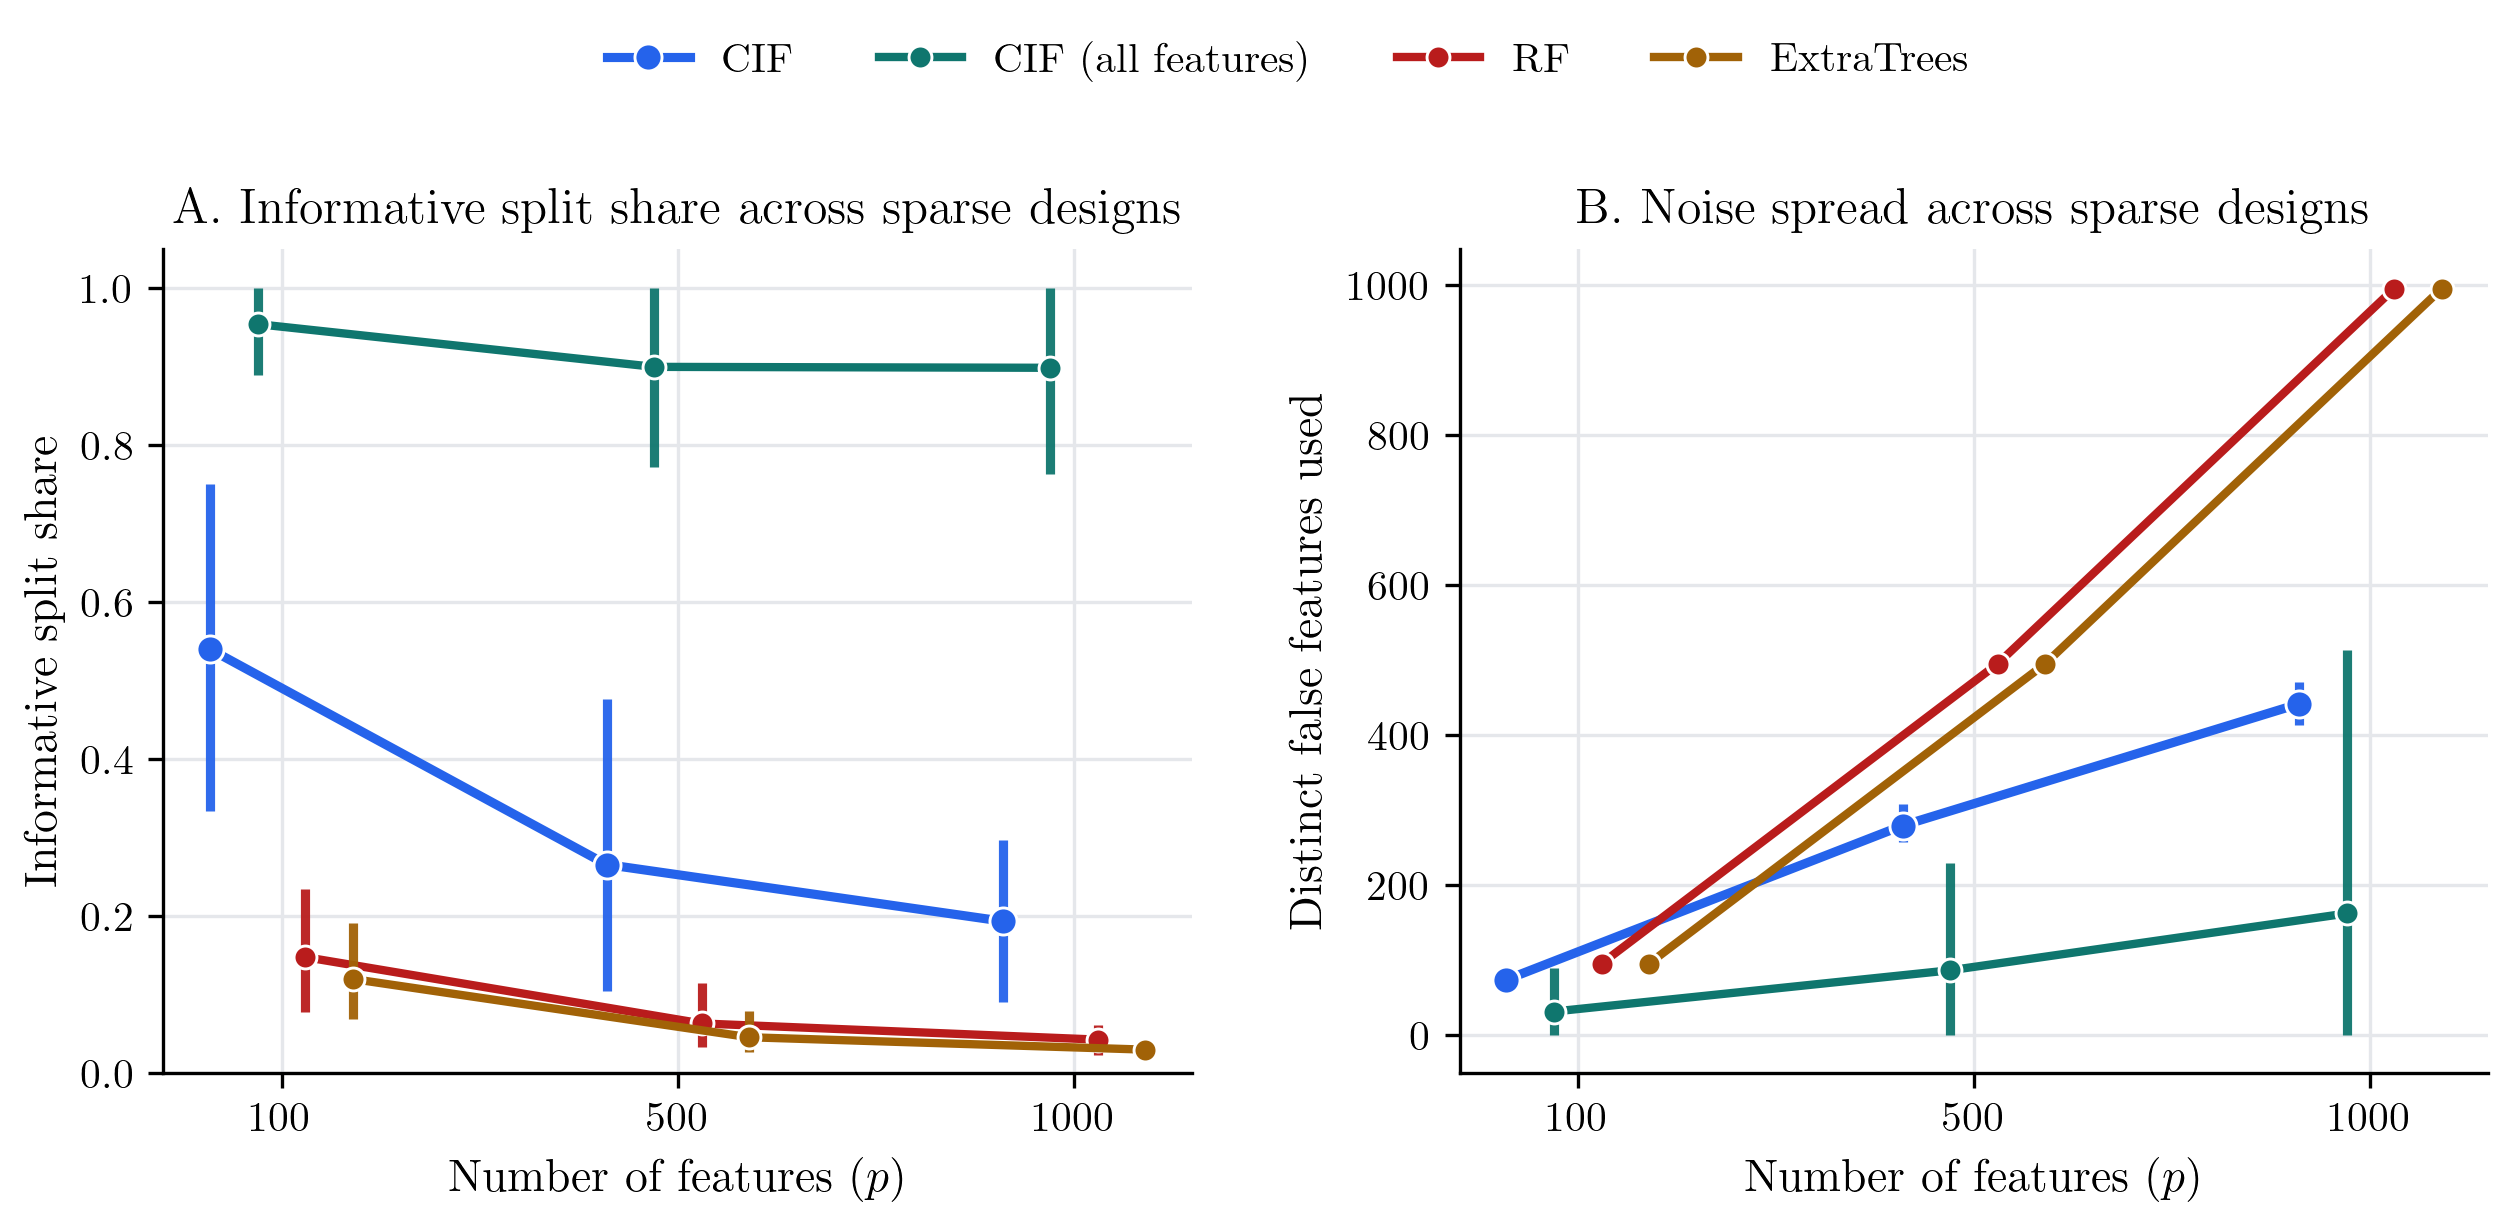
\includegraphics[width=0.88\linewidth]{figures/paper_mechanism_grid_forest_classification_dimension_curves_1000trees.png}
  \caption{Classification forest feature sampling by feature dimension
  $p$ with 1,000 trees per fit. Points are means over
  $n_{\mathrm{informative}} \in \{1,2,5,10\}$; capped bars span the
  minimum-to-maximum values across those four sparse designs.
  (A) shows \% of splits using informative features; (B) shows
  the number of distinct uninformative features used.}
  \label{fig:candidate-dimension-curves}
\end{figure}

\begin{figure}[!htbp]
  \centering
  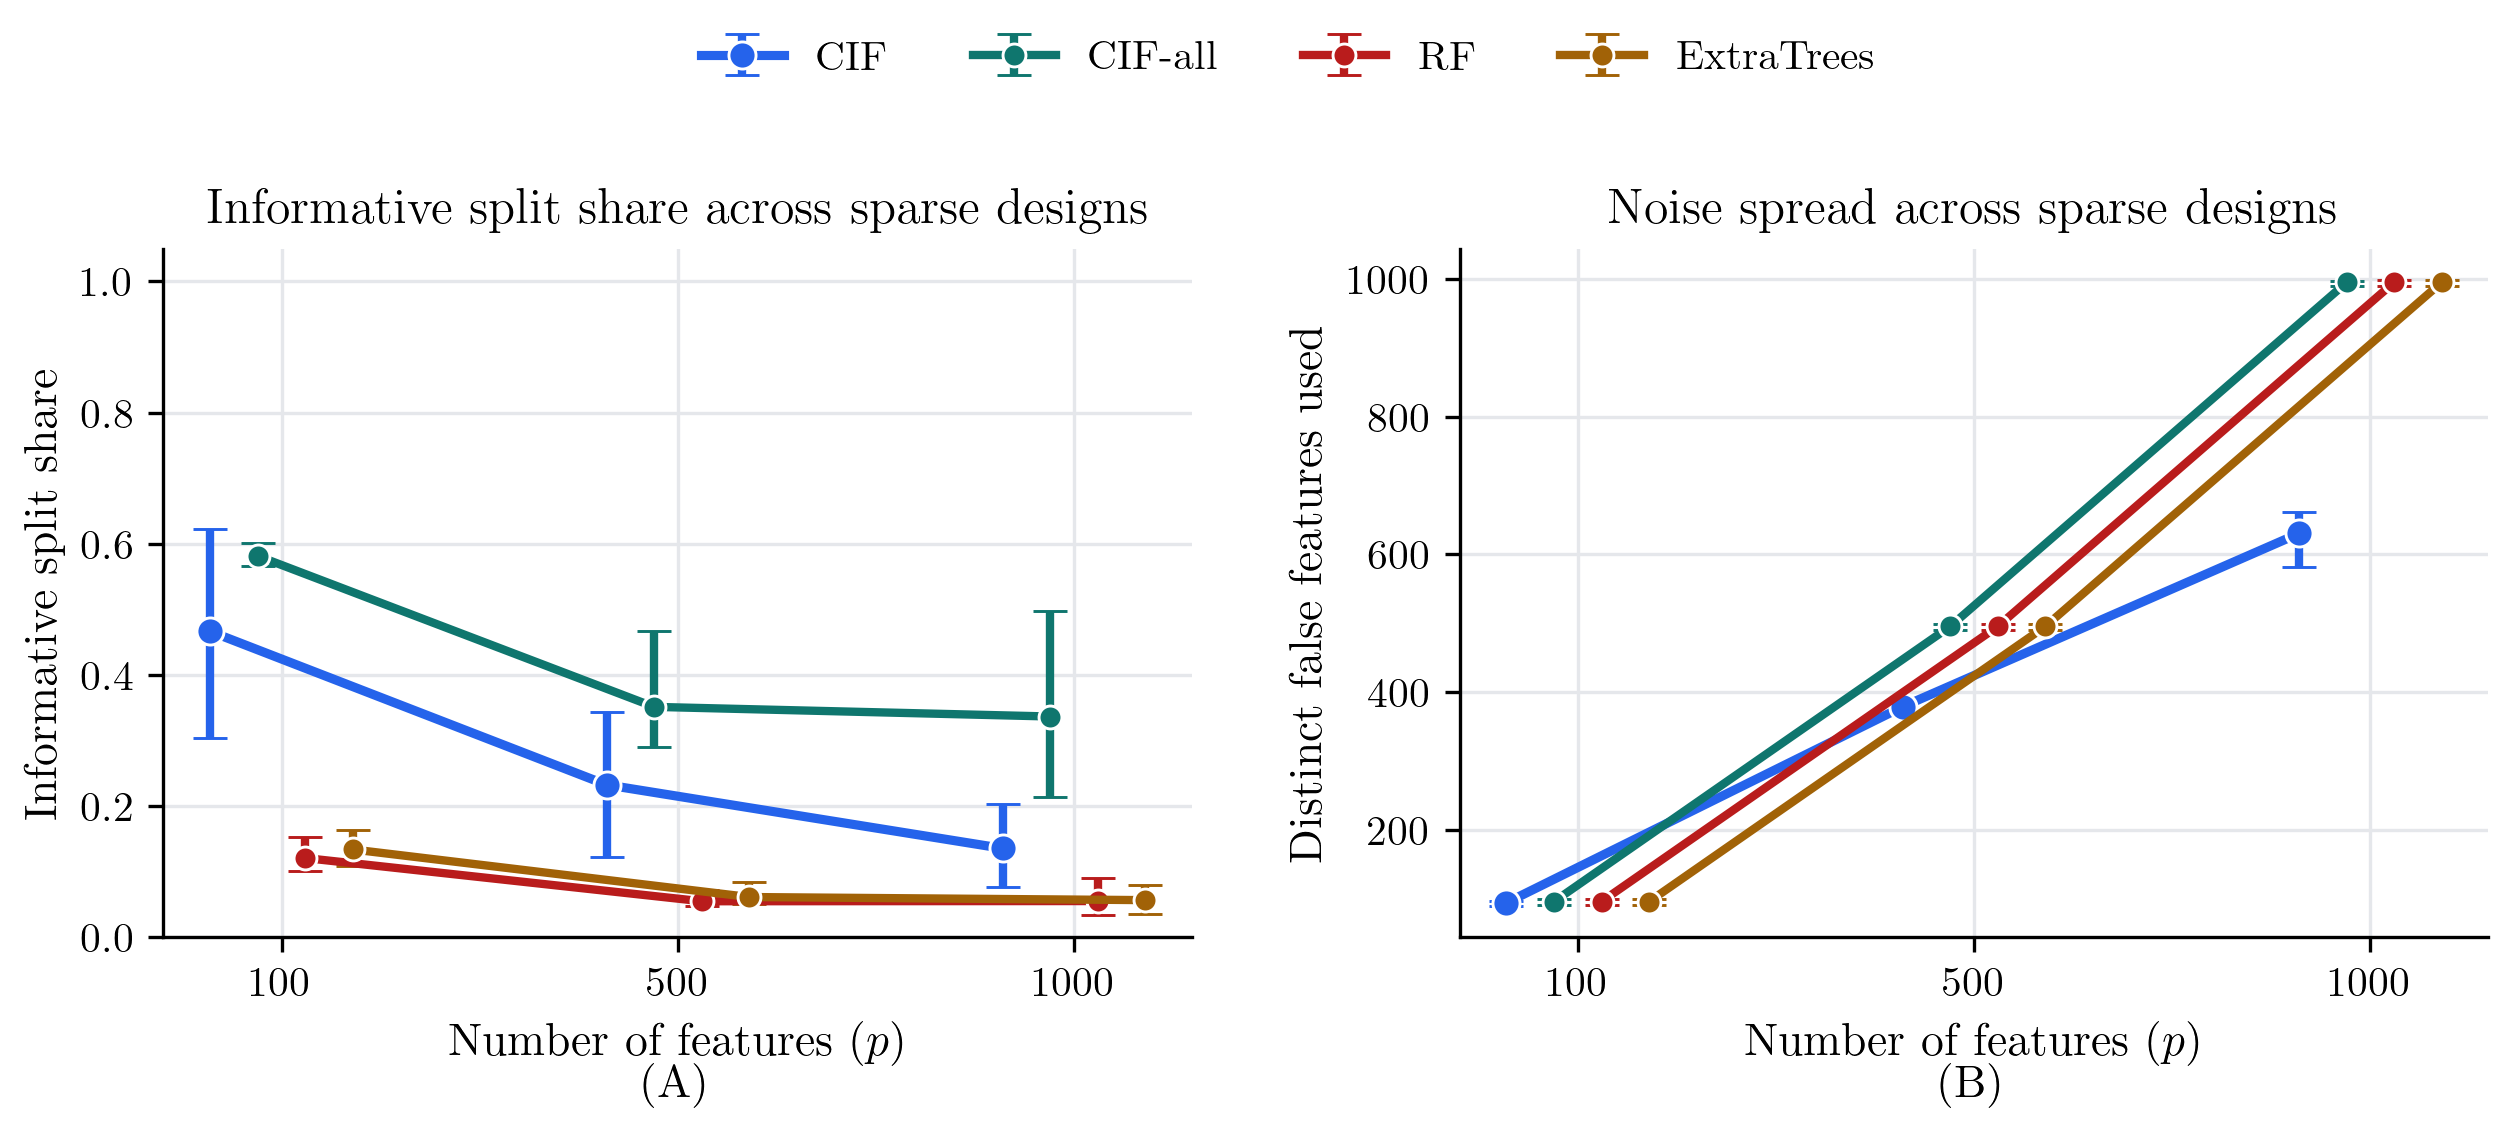
\includegraphics[width=0.88\linewidth]{figures/paper_mechanism_grid_forest_regression_dimension_curves_1000trees.png}
  \caption{Regression forest feature sampling by feature dimension
  $p$ with 1,000 trees per fit. Points are means over
  $n_{\mathrm{informative}} \in \{1,2,5,10\}$; capped bars span the
  minimum-to-maximum values across those four sparse designs.
  (A) shows \% of splits using informative features; (B) shows
  the number of distinct uninformative features used.}
  \label{fig:regression-candidate-dimension-curves}
\end{figure}
